\section[Swing komponenter]{Tilpassede \emph{Swing} komponenter} \label{sec:swing}
I programmet er det brukt flere spesialtipassede komponenter arvet fra swing klassen med spesiltipasninger f.eks for størrelse, brukerinteraksjon eller andre tilpassninger. Komponentene er plassert i pakke \texttt{view} og \texttt{view.register}.

\subsection{\texttt{AbstractPanel.java}}
Abstract panel som arver \texttt{JPanel} er klassen som ligger til grunn til alle paneler som er i bruk i programmet. Klassen har to konstruktører og har som regel følgende oppgaver:
\begin{itemize}
\item Setter størrelse (dimensjon) på panelen.
\item Setter bakgrunnfarve på panelen fra gn global static konstant. Dette gjør at farve på all brukegrensesnitt i programmet kan enkelt endres.
\item Sette en \texttt{titleBorder} rundt komponenten fra parameter i konstruktøren. Avhengig av hvilken kontsruktør som brukes.
\end{itemize}
Dimensjonen settes gjennom å kalle opp metoden \texttt{setPrefferedSize(Dim dim)} som brukes ettersom slik tilnærming gjør at størrelse på panelen blir "<respektert"> av valgt layout manager (dette gjelder ikek altid dersom \texttt{setSize()} brukes.





\subsection{\texttt{AbstraktArkfane.java}}
Abstract klasse som arver \texttt{AbstractPanel}. Klassen som arver den får et oppsett av paneler. Hvilket oppsett av paneler som blir oprettet er avhengig av hilken parameter som blir sendt inn i konstruktøren se eksempel +ref{kode:arkfane}. Hvilke type av arkfane som skal bli oprettet bestemmes a streg parametern som blir sendt inn til konstruktøren. Klassen arves av to klasser: \texttt{ArkfaneMegler.java} og \texttt{ArkfaneAnnonse.java} hvilke setter begge faner i programmet. 

\begin{lstlisting}[caption=Konstruktør til \texttt{AbstraktArkfane}. label=kode:arkfane]
    public AbstraktArkfane(String valgtToppanel) {
        setLayout(new BorderLayout());
        setVisible(true);
        
        bunnpanel = new BunnPanel(VinduStorrelse.BUNNPANEL.getHEIGHT(), 
                VinduStorrelse.BUNNPANEL.getWIDTH());
        venstrepanel = new VenstrePanel("Liste",VinduStorrelse.VENSTREPANEL.getHEIGHT(), 
                VinduStorrelse.VENSTREPANEL.getWIDTH());
        senterpanel = new SenterPanel("Visning",VinduStorrelse.SENTERPANEL.getHEIGHT(), 
                VinduStorrelse.SENTERPANEL.getWIDTH());

        if (valgtToppanel.equals("megler")) {
            toppanel = new TopPanelMegler("Søk",VinduStorrelse.TOPPANEL.getHEIGHT(), 
                    VinduStorrelse.TOPPANEL.getWIDTH());
            add(toppanel, BorderLayout.NORTH);
        } else{
            toppanel = new TopPanelAnnonse("Søk",VinduStorrelse.TOPPANEL.getHEIGHT(), 
                    VinduStorrelse.TOPPANEL.getWIDTH());
            add(toppanel, BorderLayout.NORTH);
        }
        add(venstrepanel, BorderLayout.WEST);
        add(senterpanel, BorderLayout.CENTER);
        add(bunnpanel, BorderLayout.SOUTH);
    }
\end{lstlisting}


\begin{figure}[ht]
 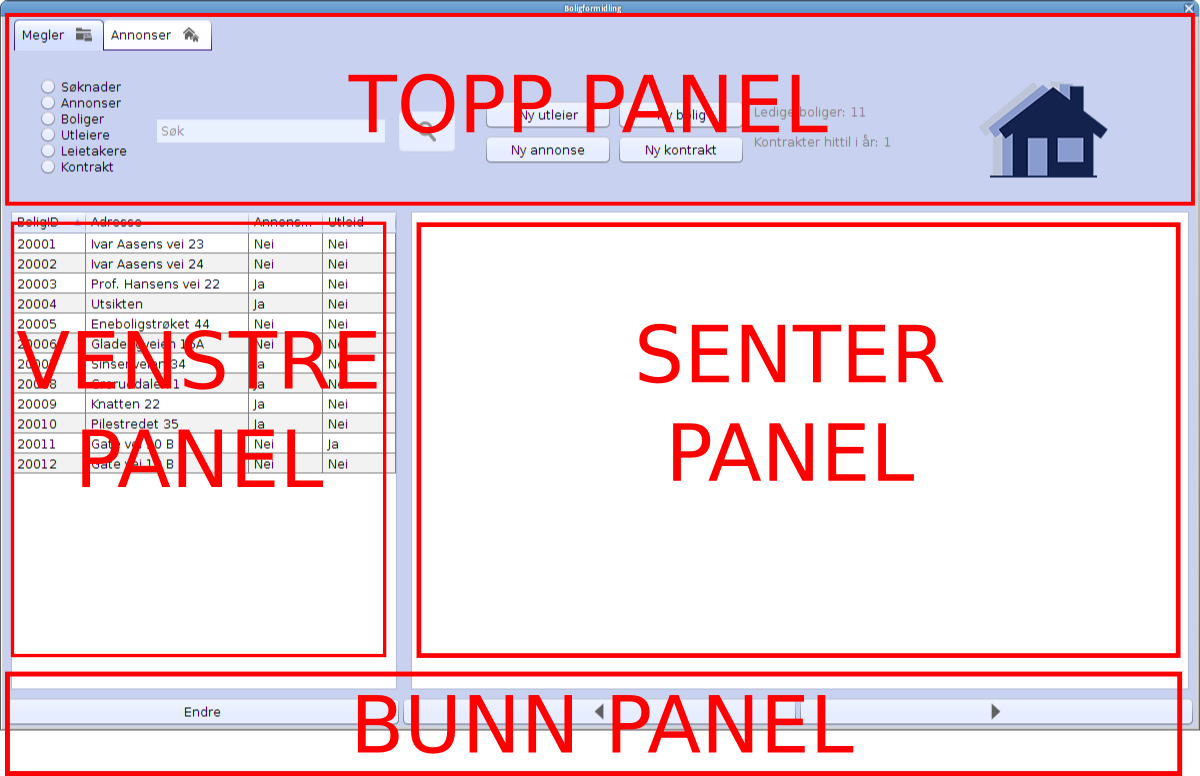
\includegraphics[width=\textwidth,height=\textheight,keepaspectratio]{./img/produktdokumentasjon/swing_componenter/AbstraktArkfane.png}
 \caption{Fordeling mellom komponenter i AbstraktArkfane}
 \label{fig:asbtarkfane}
\end{figure}



\subsection{\texttt{CustomJTextField.java}}
\texttt{CustomJTextFiled} arver \texttt{AbstractPanel} og dermed innholder samme konstruktør som denne panelen hvilken setter feltets dimensjoner. Slik løsning medfører også at hvert tekstfelt er plasser i en egen \texttt{JPanel}\footnote{arves av \texttt{AbstractPanel}}.
Tekstfeltet er spesiltipasset slik at en den innholder en indre label som kan for eksempel brukes til å sette en mal på hva brukeren skal skrive inn i tekstfeltet. Eksempelvis kan dette være forventet antall sifferer i et telefon- eller personnummer, figur \ref{fig:custom1}. Feltet innholder også to lytter for \texttt{focusEvent} som initialiserer en regex etter en regex mønster som settes via feltets kontruktør. Regex mønster hentes via static konstant som passer et uttrykk som feltet skal brukes til (se avsnitt \ref{subsec:regextest}, side \pageref{subsec:regextest}). Etter at markøren flyttes ut fra feltet hvis da regex testen feilr blir feltet markert med rød farve som det vises i figur \ref{fig:custom2}.
Panelen overrider også de metoder som man ønsker at skal være tilgjengelige fra superklassen \texttt{JTextField} som er \texttt{getText()}, \texttt{setText()} og \texttt{setEnabled()}.

\begin{figure}[ht!]
\centering
\begin{subfigure}[b]{1\textwidth}
\centering


\includegraphics[scale=0.7]{./img/produktdokumentasjon/swing_componenter/1.png}
\caption{Inaktiv, indre label}
\label{fig:custom1}
\end{subfigure}
\quad

\begin{subfigure}[b]{1\textwidth}
\centering

\includegraphics[scale=0.7]{./img/produktdokumentasjon/swing_componenter/2.png}
\caption{Regex kontroll feilet}
\label{fig:custom2}
\end{subfigure}
\quad

\caption{Forsjellige tilstand av CustomJPane}\label{fig:customjpane}
\end{figure}